%% 
%% Copyright 2019-2024 Elsevier Ltd
%% 
%% Version 2.4
%% 
%% This file is part of the 'CAS Bundle'.
%% --------------------------------------
%% 
%% It may be distributed under the conditions of the LaTeX Project Public
%% License, either version 1.2 of this license or (at your option) any
%% later version.  The latest version of this license is in
%%    http://www.latex-project.org/lppl.txt
%% and version 1.2 or later is part of all distributions of LaTeX
%% version 1999/12/01 or later.
%% 
%% The list of all files belonging to the 'CAS Bundle' is
%% given in the file `manifest.txt'.
%% 
%% Template article for cas-dc documentclass for 
%% double column output.

%\documentclass[a4paper,fleqn,longmktitle]{cas-dc}
\documentclass[a4paper,fleqn]{cas-dc}

%\usepackage[authoryear,longnamesfirst]{natbib}
%\usepackage[authoryear]{natbib}
\usepackage[numbers]{natbib}

%% The amssymb package provides various useful mathematical symbols
\usepackage{amssymb}
\usepackage{hyperref}
\usepackage{amsmath}
\usepackage{caption}

%%%Author definitions
\def\tsc#1{\csdef{#1}{\textsc{\lowercase{#1}}\xspace}}
\tsc{WGM}
\tsc{QE}
\tsc{EP}
\tsc{PMS}
\tsc{BEC}
\tsc{DE}
%%%

\begin{document}
\let\WriteBookmarks\relax
\def\floatpagepagefraction{1}
\def\textpagefraction{.001}
\shorttitle{Utilization of environmental and epidemiological indicators in the study of malaria dynamics}
\shortauthors{R. F. Levy et~al.}

\title [mode = title]{Utilization of environmental and epidemiological indicators in the study of malaria dynamics}                      

%%%%% FOOTNOTES %%%%%
%\tnotemark[1,2]

%%%%% FOOTNOTES %%%%%
%\tnotetext[1]{This document is the results of the research
%   project funded by the National Science Foundation.}

%\tnotetext[2]{The second title footnote which is a longer text matter
%   to fill through the whole text width and overflow into
%   another line in the footnotes area of the first page.}

\author[1]{Raphael Felberg Levy}
\ead{raphael.levy147@gmail.com}
%\author[1,3]{J.K. Krishnan}[type=editor,
%                        auid=000,bioid=1,
%                        prefix=Sir,
%                        role=Researcher,
%                       orcid=0000-0001-0000-0000]
%\cormark[1]
%\fnmark[1]
%\ead{jkk@example.in}
%\ead[url]{www.jkkrishnan.in}

%\credit{Conceptualization of this study, Methodology, Software}

%\address[1]{, Street 129, 1043 NX Amsterdam, The Netherlands}
\affiliation[1]{organization={School of Applied Mathematics, EMAp FGV},
                addressline={Praia de Botafogo 190}, 
                city={Rio de Janeiro},
%               citysep={}, % Uncomment if no comma needed between city and postcode
                postcode={22250-145}, 
                state={RJ},
                country={Brazil}}

%\author[2,4]{Han Thane}[style=chinese]
\author[1]{Flavio Codeço Coelho}
\ead{flavio.codeco.coelho@fgv.br}



%\credit{Data curation, Writing - Original draft preparation}

%\affiliation[2]{organization={World Scientific University},
%                addressline={Street 29}, 
%                postcode={1011 NX}, 
%                postcodesep={}, 
%                city={Amsterdam},
%                country={The Netherlands}}

%\author[1,3]{T. Rafeeq}
%\cormark[2]
%\fnmark[1,3]
%\ead{t.rafeeq@example.in}
%\ead[URL]{www.campus.in}

%\affiliation[3]{organization={University of Intelligent Studies},
%                addressline={Street 15}, 
%                city={Jabaldesh},
%                postcode={825001}, 
%                state={Orissa}, 
%                country={India}}

%\cortext[cor1]{Corresponding author}
%\cortext[cor2]{Principal corresponding author}
%\fntext[fn1]{This is the first author footnote, but is common to third
%  author as well.}
%\fntext[fn2]{Another author footnote, this is a very long footnote and
%  it should be a really long footnote. But this footnote is not yet
%  sufficiently long enough to make two lines of footnote text.}

%%%% FOOTNOTE %%%%
%\nonumnote{This note has no numbers. In this work we demonstrate $a_b$
%  the formation Y\_1 of a new type of polariton on the interface
%  between a cuprous oxide slab and a polystyrene micro-sphere placed
%  on the slab.
% }


\begin{abstract}
%This template helps you to create a properly formatted \LaTeX\ manuscript.
This paper aims to analyze the behavior of malaria transmission in the Amazon region based on climatic and environmental changes, such as temperature, precipitation and deforestation, through proposed modifications to the SIR and SEI models, in order to contribute to the study of applications of external effects on the evolution of the disease. 
The Trajetórias Project, developed by the Synthesis Center 
on Biodiversity and Ecosystem Services (SinBiose/CNPq) was used as an initial reference for the study. This work employs a modified SIR/SEI methodology, based on work from Parham and Michael (2010) which takes into account rainfall and temperature, with further modifications to avoid delay equations. Primary results show that the model is too sensible on some parameters, and using values indicated by other papers did not give the same results, opening up future work to compare the modified model equations with the originals. With the obtained results, it was possible to verify a strong effect caused by increased contact of host and vectors on the transmission of the disease. 

\end{abstract}


%\noindent\texttt{\textbackslash begin{abstract}} \dots 
%\texttt{\textbackslash end{abstract}} and
%\verb+\begin{keyword}+ \verb+...+ \verb+\end{keyword}+ 
%which contain the abstract and keywords respectively. 

%\noindent Each keyword shall be separated by a \verb+\sep+ command.



%\begin{graphicalabstract}
%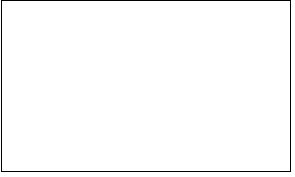
\includegraphics{figs/cas-grabs.pdf}
%\end{graphicalabstract}

%\begin{highlights}
%\item Research highlights item 1
%\item Research highlights item 2
%\item Research highlights item 3
%\end{highlights}

\begin{keywords}
Biological modelling \sep Malaria transmission \sep Climate change \sep Amazon \sep SIR \sep SEI
\end{keywords}


\maketitle

\section{Introduction}

The Amazon is one of the largest and most biodiverse tropical forests 
in the world, harboring numerous species of plants, animals, and 
microorganisms, including vectors and pathogens responsible for the 
transmission of various diseases. Among them, one of the most common 
is malaria, caused by protozoa of the genus \textit{Plasmodium}, 
transmitted by the bite of the infected female mosquito of the genus 
\textit{Anopheles}. It is present in 22 American countries, but the 
areas with the highest risk of infection are located in the Amazon 
region, encompassing nine countries, which accounted for $68\%$ of 
infection cases in 
2011 \cite{pimenta_orfano_bahia_duarte_rios-velasquez_melo_pessoa_oliveira_campos_villegas_etal_2015}. 
Although malaria is prevalent in the Americas, it is 
not limited to this continent and is found in countries in Africa and Asia, 
resulting in more than two million cases of infection and 445,000 deaths 
worldwide in 2016 \cite{regulation_of_sexual_commitment}, being endemic in a total of 84 countries in 2021 \cite{WHO2022}.

Notably, vector-borne disease transmission is closely related to 
environmental changes that interfere with the ecosystem of both 
transmitting organisms and affected organisms. In the case of the 
Amazon, agricultural and livestock settlements are among the factors
that most favor disease transmission, both due to the deforestation 
they cause for establishment and the clustering of people in environments 
close to the vector's habitat \cite{silva-nunes_malaria_amazon_2008}, 
especially by clustering non-immune migrants near these natural and 
artificial breeding sites \cite{DASILVANUNES2012281}.

Additionally, other factors such as rainfall, wildfires, and mining 
also significantly influence disease transmission in the region. These 
events result in habitat loss, ecosystem fragmentation, and climate 
changes, affecting the distribution and abundance of vectors and hosts, 
as well as their interaction with pathogens. Furthermore, population growth 
and urbanization also play a crucial role in disease spread, increasing 
human exposure to vectors and infection risks.

In this context, this work aims to investigate vector-borne disease 
transmission in the Amazon and analyze how environmental impacts 
influence the dynamics of malaria transmission, the ecological and 
socioeconomic factors affecting this spread, and possible prevention 
and control strategies. The main reference for this research is the 
Trajetórias Project, developed by the Center for Biodiversity and 
Ecosystem Services (SinBiose/CNPq), which is a dataset including 
environmental, epidemiological, economic, and socioeconomic indicators 
for all municipalities in the Legal Amazon, analyzing the spatial and 
temporal relationship between economic trajectories linked to the dynamics 
of agrarian systems, whether they are family-based rural or large-scale 
agricultural and livestock production, the availability of natural resources, 
and the risk of diseases \cite{Rorato2023}.

\section{Model formulation}

Based on previous work developed to model the transmission of malaria based on precipitation and temperature dynamics \cite{Parham2010}, we focus 
on two different sets of compartments: susceptible hosts ($S_H$), infected hosts ($I_H$), recovered hosts ($R_H$), susceptible vectors ($S_M$), 
exposed vectors ($E_M$) and infected vectors ($I_M$). The equations that describe the transmission are initially given as:
%\begin{gather}
\begin{align}
\dfrac{dS_H}{dt} & = -ab_2\bigg(\dfrac{I_M}{N}\bigg)S_H \label{eq1}\\
\dfrac{dI_H}{dt} & = ab_2\bigg(\dfrac{I_M}{N}\bigg)S_H - \gamma I_H \label{eq2}\\
\dfrac{dR_H}{dt} & = \gamma I_H \label{eq3}\\
\dfrac{dS_M}{dt} & = b - ab_1\bigg(\dfrac{I_H}{N}\bigg)S_M - \mu S_M \label{eq4}\\
\dfrac{dE_M}{dt} & = ab_1\bigg(\dfrac{I_H}{N}\bigg)S_M - \mu E_M - ab_1\bigg(\dfrac{I_H}{N}\bigg)S_Ml(\tau_M) \label{eq5}\\
\dfrac{dI_M}{dt} & = ab_1\bigg(\dfrac{I_H}{N}\bigg)S_Ml(\tau_M) - \mu I_M \label{eq6}
\end{align}
%\end{gather}

However, the use of these equations proved to be unsuccessful for the modelling of the mosquito populations through the SEI equations, 
causing $(5)$ to be very close to 0, and therefore mirroring the oscillations of $S$ and $I$, a behavior not seen in nature. 

To overcome this effect, the SEI equations were modified in order for $b_1$ to only be used in the transference between compartments $S$ and $E$, 
and a new parameter, $b_3$ to move mosquitos from $E$ to $I$. Being inversely related to the incubation period, the definition of this rate can be found in \textbf{Table A.2}. 
In addition to that, the parameter $a(T)$ that was in use in the transition between exposed and infected also had to be removed, as no further bites occur at this point.

The parameters are given in Table A1, while the variables are given in Table A2, which can be found in the Appendix. 
The selected human population was from the the rural area of Manaus, between the years of 2004 to 2008, as this locality had the highest incidence of malaria 
caused by $P. \ vivax$ in the Amazon region \cite{Rorato2023}. This species of $\text{Plasmodium}$ was chosen as it is responsible for the highest number of malaria
 cases in Brazil \cite{OliveiraFerreira2010, 10.3389/fpubh.2021.647754}, being the most common human malaria 
parasite in the region \cite{Vector_Incrimination}. With the incidence function \cite{Rorato2023} we have that

\begin{align}
\text{Inc} = %(d, m, z, t_1, t_2) = 
\dfrac{\text{Cases}(d, m, z, t_1, t_2)}{\text{Pop}(m,z,(t_1+t_2)/2) \times 5 \ \text{years}} \times 10^5,
\end{align}

where $\text{Cases}(d, m, z, t_1, t_2)$ is the number of cases of disease $d$ in zone $z$ of municipality 
$m$, and $t_1$ and $t_2$ are the initial and final years of the interval, while 
$\text{Pop}(m,z,(t_1+t_2)/2) \times 5 \ \text{years}$ is the population in zone $z$ 
of municipality $m$ in the middle of the period multiplied by the total number 
of observation years. In this case, we could indicate as:

\begin{align}
    \footnotesize{\text{Inc}(\text{Vivax}, \text{Manaus}, \text{Rural}, 2004, 2008) = } \\
= \footnotesize{\dfrac{\text{Cases}(\text{Vivax}, \text{Manaus}, \text{Rural}, 2004, 2008)}{\text{Pop}(\text{Manaus}, \text{Rural}, 2006) \times 5 \ \text{years}} \times 10^5} \Rightarrow  \\
    \Rightarrow 184030.8 = \dfrac{78745}{5\text{Pop}} \times 10^5 \Rightarrow Pop \approx 8558
\end{align}

Using data on the total population of Manaus in this period, 
with an incidence of 3106.429047 and a number of cases of 262264, the 
total population of the municipality was estimated to be 1688524 
inhabitants, which corresponds to the value found in the official census \cite{Datasus2006}. Thus, the rural population could be considered as 
approximately 0.5$\%$ of the municipality's population.

Having estimated the percentage size of the rural population 
in the city, it was possible to calculate this population for 
each of the years of the analysis through linear interpolation 
using historical series data from IBGE \cite{popIBGE}:

\begin{table}[width=.9\linewidth,cols=4,pos=h]
\caption{Manaus' rural population from 2004 to 2009.}\label{tbl1}
\begin{tabular*}{\tblwidth}{@{} LL@{} } %| L | L | L | L |
\toprule
\textbf{Year}  & \textbf{Estimated rural population}\\
\midrule
$2004$ & $7717$ \\
 $2005$ & $7889$ \\
$2006$ & $8061$ \\
$2007$ & $8233$ \\
$2008$ & $8492$ \\
$2009$ & $8751$ \\
\bottomrule
\end{tabular*}
\end{table}


%\begin{table}[h]
%\caption{Manaus' rural population from 2004 to 2009.}
%\centering
%\begin{tabular}{|c | c|}
 %\hline
 %\textbf{Year} & \textbf{Estimated rural population}\\ 
% \hline
%$2004$ & $7717$ \\
% \hline
%$ $2005$ & $7889$ \\
 %\hline
% $2006$ & $8061$ \\
% \hline
 %$2007$ & $8233$ \\
 %\hline
% $2008$ & $8492$ \\
% \hline
% $2009$ & $8751$ \\
% \hline
%\end{tabular}
%\end{table}
Given there was only population data for the years of 2000, 2007, and 2010, 
interpolations were performed with different initial and final 
points, using data from 2000 to 2007 for 2004-2007 and from 2007 
to 2010 for 2008-2009, ensuring the correct use of the 2007 population.

Temperature and precipitation data were taken from the Mosqlimate Data API datastore \cite{MosqlimateAPI}, from January 1st 2004 to December 31st 2008, with the geocode 1302603.

As for the theory behind environmental factors, it is known that the removal of tree canopies allowed 
the resurgence of malaria in South America \cite{Norris2004}. In deforested areas, 
without tree canopies covering the ground, water puddles under sunlight 
attract mosquitoes of the species $Anopheles \ darlingi$, the main vector 
related to human malaria in the Amazon \cite{infoAnopheles}. They are 
usually less commonly found in still intact forests. This is 
because light and heat favor the development of larvae and 
pupae, in addition to a greater availability of algae for 
larval feeding \cite{article_alteracoesambientais}. The increase 
in ambient temperature also favors the vectorial capacity of 
mosquitoes. 

Deforestation also attracts and brings humans closer 
to take part in logging, agriculture, and road construction 
activities, bringing individuals infected with $Plasmodium$ to 
an area where both the vector and the environment have already 
been modified to favor transmission. Furthermore, agriculture 
also promotes river sedimentation, providing suitable environments 
for breeding sites. Therefore, it can be considered a relevant 
change for the model to take into account deforestation, the 
increase in survival probabilities of eggs, larvae, and pupae, 
as well as increasing the proportion of bites that lead to infection, 
due to the increased human population density in areas near mosquito 
breeding sites.

As it was outside the scope of this project to collect samples of $A. \ darlingi \ in \ loco$, it was instead used 
an estimate for the number of mosquitos based in the literature. As the study was made around the rural population of the municipality,
this would favour the clustering of adult mosquitos, given the proximity to bodies of water and recently open up areas of rainforest \cite{Biological_Variation_Anopheles}.

 \begin{thebibliography}{00}

%% \bibitem must have the following form:
%%   \bibitem{key}...
%%

%1
\bibitem{pimenta_orfano_bahia_duarte_rios-velasquez_melo_pessoa_oliveira_campos_villegas_etal_2015} P.F.P. Pimenta et al., An overview of malaria transmission from the perspective of Amazon \emph{Anopheles vectors}, Memórias do Instituto Oswaldo Cruz, Vol. 110 (1) (2015), 23-47, \href{https://doi.org/10.1590/0074-02760140266}{https://doi.org/10.1590/0074-02760140266}.
\\
%2
\bibitem{regulation_of_sexual_commitment} G.A. Josling, K.C Williamson, M. Llinás, Regulation of Sexual Commitment and Gametocytogenesis in Malaria Parasites, Annual Review of Microbiology, Vol. 72 (1) (2018), 501-519, \href{https://doi.org/10.1146/annurev-micro-090817-062712}{https://doi.org/10.1146/annurev-micro-090817-062712}.
\\
%3
\bibitem{WHO2022} World Health Organization / World Malaria Report 2022, Global Malaria Programme, accessed 29 August 2024, \href{https://www.who.int/publications/i/item/9789240064898}{https://www.who.int/publications/i/item/9789240064898}.
\\
%4
\bibitem{silva-nunes_malaria_amazon_2008} M. Silva-Nunes et al., Malaria on the Amazonian frontier: transmission dynamics, risk factors, spatial distribution, and prospects for control, American Journal of Tropical Medicine and Hygiene, Vol. 79 (4) (2008), 624-635, \href{https://doi.org/10.4269/ajtmh.2008.79.624}{https://doi.org/10.4269/ajtmh.2008.79.624}. 
\\
%5
\bibitem{DASILVANUNES2012281} M. Silva-Nunes et al.,  Amazonian malaria: Asymptomatic human reservoirs, diagnostic challenges, environmentally driven changes in mosquito vector populations, and the mandate for sustainable control strategies, Acta Tropica, Vol. 121 (3) (2012), 281-291 , \href{https://doi.org/10.1016/j.actatropica.2011.10.001}{https://doi.org/10.1016/j.actatropica.2011.10.001}.
\\
%6
\bibitem{Rorato2023} A.C. Rorato, A.P. Dal’Asta, R.M. Lana et al., Trajetorias: a dataset of environmental, epidemiological, and economic indicators for the Brazilian Amazon, Scientific Data, Vol. 10 (1) (2023), 65, \href{https://doi.org/10.1038/s41597-023-01962-1}{https://doi.org/10.1038/s41597-023-01962-1}.
\\
%7
\bibitem{Parham2010} P.E.Parham, E. Michael, Modelling Climate Change and Malaria Transmission, Modelling Parasite Transmission and Control, Advances in Experimental Medicine and Biology, Vol. 673 (2010), 184-199, \href{https://doi.org/10.1007/978-1-4419-6064-1_13}{https://doi.org/10.1007/978-1-4419-6064-1\_13}.
\\
%8
\bibitem{McCord2016} G.C. McCord, Malaria ecology and climate change, The European Physical Journal Special Topics, Vol. 225 (3) (2016), 459-470, \href{https://doi.org/10.1140/epjst/e2015-50097-1}{https://doi.org/10.1140/epjst/e2015-50097-1}.
\\
%9
\bibitem{Lindsay_Birley_1996} S. W. Lindsay, M. H. Birley, Climate change and malaria transmission, Annals of Tropical Medicine \& Parasitology,Vol. 90 (1996), 573-588, \href{https://doi.org/10.1080/00034983.1996.11813087}{https://doi.org/10.1080/00034983.1996.11813087}.
\\
%10
\bibitem{OliveiraFerreira2010} J. Oliveira-Ferreira, M. V. Lacerda, P. Brasil et al., Malaria in Brazil: an overview., Malaria Journal, Vol. 9 (1) (2010), \href{https://doi.org/10.1186/1475-2875-9-115}{https://doi.org/10.1186/1475-2875-9-115}.
\\
%11
\bibitem{10.3389/fpubh.2021.647754} C.T. Codeço, A.P. Dal'Asta, A.C. Rorato, R.M. Lana, T.C. Neves, C.S. Andreazzi, M. Barbosa, M.I.S. Escada, D.A. Fernandes, D.L. Rodrigues, I.C. Reis, M. Silva-Nunes, A.B. Gontijo, F.C. Coelho, A.M.V. Monteiro, Epidemiology, Biodiversity, and Technological Trajectories in the Brazilian Amazon: From Malaria to COVID-19, Frontiers in Public Health, Vol. 9 (2021), \href{https://doi.org/10.3389/fpubh.2021.647754}{https://doi.org/10.3389/fpubh.2021.647754}.
\\
%12
\bibitem{Vector_Incrimination} A. K. R. Galardo, M. Arruda, et al., Malaria vector incrimination in three rural riverine villages in the Brazilian Amazon, The American Journal of Tropical Medicine and Hygiene, Vol. 76 (3) (2007), 461-469, \href{https://www.ajtmh.org/view/journals/tpmd/76/3/article-p461.xml}{https://www.ajtmh.org/view/journals/tpmd/76/3/article-p461.xml}.
\\
%13
\bibitem{Datasus2006} Tabnet, Ministério da Saúde, accessed 12 August 2024, \href{http://tabnet.datasus.gov.br/cgi/tabcgi.exe?ibge/cnv/popam.def}{http://tabnet.datasus.gov.br/cgi/tabcgi.exe?ibge/cnv/popam.def}.
\\
%14
\bibitem{popIBGE} Censo - Séries históricas. Brasil / Amazonas / Manaus, IBGE, accessed 15 August 2024, \href{https://cidades.ibge.gov.br/brasil/am/manaus/pesquisa/43/0?tipo=grafico}{https://cidades.ibge.gov.br/brasil/am/manaus/pesquisa/43/0?tipo=grafico}.
\\
%15
\bibitem{MosqlimateAPI} Mosqlimate Data API / Datastore / climate, accessed 12 August 2024, \href{https://api.mosqlimate.org/datastore/}{https://api.mosqlimate.org/datastore/}.
\\
%16
\bibitem{Norris2004} D. E. Norris, Mosquito-borne Diseases as a Consequence of Land Use Change, EcoHealth, Vol. 1 (1) (2004), 19-24, \href{https://doi.org/10.1007/s10393-004-0008-7}{https://doi.org/10.1007/s10393-004-0008-7}.
\\
%17
\bibitem{infoAnopheles} Anopheles, Fiocruz Rondônia, accessed 15 August 2024, \href{https://www.rondonia.fiocruz.br/pivem/anopheline/}{https://www.rondonia.fiocruz.br/pivem/anopheline/}.
\\
%18
\bibitem{article_alteracoesambientais} M. Silva-Nunes, Environmental changes impact in malaria transmition and prospects for the disease control in brazilian amazon rural settlements, Oecologia Australis, Vol. 14 (3) (2010), 603-622, \href{https://revistas.ufrj.br/index.php/oa/article/view/7101}{https://revistas.ufrj.br/index.php/oa/article/view/7101}.
\\
%19
\bibitem{Biological_Variation_Anopheles} J. D. Charlwood, Biological variation in Anopheles darlingi Root, Memórias do Instituto Oswaldo Cruz, Vol. 91 (4) (1996), 391-398, \href{ https://doi.org/10.1590/S0074-02761996000400001}{ https://doi.org/10.1590/S0074-02761996000400001}.
\\

\end{thebibliography}

\clearpage

\appendix
\renewcommand{\thetable}{A.\arabic{table}}
\setcounter{table}{0}  % Restart the table counter

\section{Appendix}
%Appendix sections are coded under \verb+\appendix+.

\begin{table}[width=2.0\linewidth,cols=3,pos=h]
\caption{List of model parameters.}\label{tbl1}
\renewcommand{\thetable}{Appendix 1}  % Custom table name
\begin{tabular*}{\tblwidth}{@{} LLL@{} }
\toprule
Parameter & Definition & Formulation\\
\midrule
$b(R, T)$   & Mosquito birth rate (days$^{-1}$)   & ${B_E  p_E(R)  p_L(R,T)  p_P(R)}/{(\tau_E + \tau_L(T) + \tau_P)}$   \\ 
$a(T)$   & Biting rate (days$^{-1}$)  & ${(T - T_1)}/{D_1}$   \\ 
$\mu(T)$   & Mosquito mortality rate per capita (days$^{-1}$)   & $-\log(p(T))$  \\ 
$\tau_M(T)$   & Duration of sporozoite cycle (days)   & ${DD}/{(T - T_{min})}$   \\ 
$\tau_L(T)$   & Duration of larval development phase (days)   & ${1}/{c_1T + c_2}$  \\ 
$p(T)$   & Daily mosquito survival rate   & $e^{(-1 / (AT^2 + BT + C))}$ \\  
$p_L(R)$   & Probability of larval survival dependent on rainfall   & $({4p_{ML}}/{R_L^2})R(R_L - R)$  \\  
$p_L(T)$   & Probability of larval survival dependent on temperature   & $e^{-(c_1T + c_2)}$  \\ 
$p_L(R, T))$   &Probability of larval survival   & $p_L(R)p_L(T)$   \\  
$l({\tau_M})(T)$   &  Probability of mosquito survival during sporozoite cycle (days$^{-1}$)  & $p(T)^{\tau_M(T)}$  \\ 
$M(t)$   &  Total population of mosquitos  & $S_M(t) + E_M(t) + I_M(t)$   \\ 
$N(t)$   & Total population of humans   & $S_H(t) + I_H(t) + R_H(t)$   \\ 
\bottomrule
\end{tabular*}
\end{table}

%\clearpage

\begin{table}[width=2.0\linewidth,cols=3,pos=h]
\caption{List of model variables.}\label{tbl2}
\renewcommand{\thetable}{Appendix 2}  % Custom table name
\begin{tabular*}{\tblwidth}{@{} LLL@{} }
\toprule
Symbol & Definition & Units \\
\midrule
$b_1$  & Proportion of bites from susceptible mosquitoes on infected humans that result in infection & Dimensionless \\
$b_2$   & Proportion of bites from infected mosquitoes on susceptible humans that result in infection & Dimensionless \\
$\gamma$ &  1/Average duration of infectiousness in humans & days$^{-1}$  \\
$T_1$  & Mean temperature in the absence of seasonality & $^\circ C$ \\ 
$T_2$  & Amplitude of seasonal variability in temperature & Dimensionless \\ 
$R_1$  & Average monthly precipitation in the absence of seasonality & mm \\ 
$R_2$  & Amplitude of seasonal variability in precipitation & Dimensionless \\ 
$\omega_1$  & Angular frequency of seasonal oscillations in temperature & months$^{-1}$ \\ 
$\omega_2$  & Angular frequency of seasonal oscillations in precipitation & months$^{-1}$ \\ 
$\phi_1$  & Phase lag of temperature variability (phase shift) & Dimensionless \\ 
$\phi_2$  & Phase lag of precipitation variability (phase shift) & Dimensionless \\ 
$B_E$  & Number of eggs laid per adult per oviposition & Dimensionless \\ 
$p_{ME}$  & Maximum probability of egg survival & Dimensionless \\ 
$p_{ML}$  & Maximum probability of larval survival & Dimensionless \\ 
$p_{MP}$  & Maximum probability of pupal survival & Dimensionless \\ 
$\tau_E$  & Duration of the egg development phase & days \\ 
$b_3$  & Infection rate in exposed mosquitoes ($1/\tau_M(T)$) &  days$^{-1}$ \\ 
$\tau_P$  & Duration of the pupal development phase & days \\ 
$R_L$  & Rainfall threshold until breeding sites are eliminated, removing immature individuals & mm \\ 
$T_{min}$  & Minimum temperature, below which there is no development of the parasite: 14.5 & $^\circ C$ \\ 
$DD$  & Degree-days for parasite development.
             ``Sum of heat" for maturation: 105 \cite{McCord2016, Lindsay_Birley_1996} & $^\circ C \ \text{days}$ \\ 
$A$  & Empirical sensitivity parameter & ($^\circ C^2 \ \text{days})^{-1}$ \\ 
$B$  & Empirical sensitivity parameter & ($^\circ C \ \text{days})^{-1}$ \\ 
$C$  & Empirical sensitivity parameter & days$^{-1}$ \\ 
$D_1$  & Empirical sensitivity parameter: 36.5 & $^\circ C \ \text{days}$ \\ 
$c_1$  & Empirical sensitivity parameter & $(^\circ C \ \text{days})^{-1}$ \\ 
$c_2$  & Empirical sensitivity parameter & days$^{-1}$ \\ 
$T'$  & Empirical temperature parameter & $^\circ C$ \\ 
\bottomrule
\end{tabular*}
\end{table}

%%%%AAAA
\printcredits

%% Loading bibliography style file
%\bibliographystyle{model1-num-names}
\bibliographystyle{cas-model2-names}

% Loading bibliography database
\bibliography{cas-refs}


%\vskip3pt



\end{document}

